\documentclass[12pt]{article}
\usepackage[latin1]{inputenc}
\usepackage[paper=a4paper,dvips,top=3cm,left=3cm,right=3cm, foot=1cm,bottom=3cm]{geometry}
\usepackage{picinpar}
\usepackage{graphicx} %Graphics package for \includegraphics
\usepackage{caption}
\usepackage{subcaption}
\usepackage{wrapfig} %Enables wrapping of text around figures and tables
\usepackage{subfig}
\usepackage{enumerate}
\usepackage{multirow}
\usepackage{SIunits}%SI unit symbol package
\usepackage{amsmath}
\usepackage{array}
\usepackage{array, calc}
\usepackage{tabularx}
\usepackage{setspace}
\usepackage{verbatim} %Enables \begin{comment}...
\usepackage{cite}
\usepackage{booktabs}
\usepackage{float}
\usepackage{mathtools}
\usepackage{threeparttable}
\usepackage{standalone}
\usepackage{booktabs, dcolumn}
\usepackage{placeins}
\usepackage{inputenc} 
\usepackage{acronym}
\usepackage{placeins}

\usepackage{fancyvrb}



\tolerance = 5000 % LaTeX er normalt streng n�r det gjelder linjebrytingen.
\hbadness = \tolerance % Vi vil v�re litt mildere, s�rlig fordi norsk har s�
\pretolerance = 2000 % mange lange sammensatte ord.


\usepackage{afterpage}
\newcommand\blankpage{%
    \null
    \thispagestyle{empty}%
    \addtocounter{page}{-1}%
    \newpage}


%\newenvironment{packed_enum}{
%\newenvironment{enumerate}{
%\begin{enumerate}
  \setlength{\itemsep}{10cm}
  \setlength{\parskip}{18pt}
  \setlength{\parsep}{10pt}
%}{\end{enumerate}}


\usepackage{nomencl}
\makenomenclature
\renewcommand{\nomname}{Abbreviations}


\providecommand{\e}[1]{\ensuremath{\times 10^{#1}}}

\begin{document}

%Forside
\thispagestyle{empty}
\begin{center}        
  \vspace{5mm}        
  \huge
  \textbf{RCU2 testing and design} \\
  \vspace{50mm}
  \Large
  {\bf{\textsl{Inge Nikolai Torsvik}}} \\
  %\textsl{Eksperimentalfysikk med prosjektoppgave} \\
  \vspace{20mm}
  %{\bf{\textsl{Oppgave 12}}} \\
  \vspace{5mm}
  %{\large \textsl {(Bachelor i Fysikk)}}\\
  \vspace{10mm}
  \centerline{\includegraphics[height=4cm,width=4cm]{uiblogo.pdf}}
  \Large
  \textsl{Master Thesis} \\
  \vspace{50mm}
  \large
  \textsl{Department of Physics and Technology} \\
  \textsl{University of Bergen} \\
  \vspace{10mm}
  \large
  \textsl{November 2013} \\

\end{center}

\newpage
\blankpage
%\thispagestyle{empty}


\newpage
\setcounter{page}{1}
%\pagenumbering{roman}
\section{Abstract}

\newpage
\section{Contents}

\newpage

\section*{Acronyms}

\begin{table}[!htbp]
\begin{tabular}{ll}
\textbf{OCL} & Oslo Cyclotron Laboratory\\
\textbf{UiB} & University of Bergen\\
\textbf{UiO} & University of Oslo\\
\textbf{DUT} &  Device Under Test\\
\textbf{RAM}  & Random Access Memory\\
\textbf{SRAM} &	 \\
\textbf{FPGA} &  \\
\textbf{SC} &  \\
\textbf{SEU} &  \\
\textbf{BE} &  \\
\textbf{IC} &  \\ 
\textbf{PCB} &  \\ 
\textbf{RAM} &  \\
\textbf{RAM} &  \\
LVDS


\end{tabular}
\label{acronym}
\end{table}


\acrodef{ocl}[OCL]{Oslo Cyclotron Laboratory}
\acrodef{uib}[UiB]{University in Bergen}
\acrodef{dut}[DUT]{Device Under Test}




\newpage
\section{Introduction}

\newpage
\section{Testing at Oslo Cyclotron Laboratory(OCL)}
Every radiation tests are done at Oslo Cyclotron Laboratory at the university of Oslo.

\subsection{About OCL}
Oslo cyclotron Laboratory is located at the Department of physics at the University of Oslo, and was opened in 1978. The cyclotron is of the type MC-35 and was made by Scanditronix AB from Sweden.
This is the only accelerator in Norway for ionized atoms used in basic research.
The cyclotron can accelerate protons, Deuteron, $^3He$ and $^4He$, 
with energies and intensities as seen in the table \ref{design requirements} bellow.
A drawing of the lab can be seen bellow in figure \ref{OCL}. 
The laboratory is divided in tree; the control room, the inner experimental hall and the outer experimental hall.
The cyclotron is placed in the inner hall, and a beam is sent through pipes to the outer hall.
There is vacuum inside the cyclotron and the pipes that leads to the test area
so that you should not suffer energy loss from collision with air molecules.
With magnet you are able to regulate the beam, so that you are able to get the beam to your desired pipe exit.
There are also several cups put on the pipeline, that you are able to block the beam.
These can be used to stop the beam during an experiment, so you are able to go into the experimental area and do changes on your setup.
When the cyclotron is running and the beam is on, you are not allowed to enter the inner experimental area.

\begin{figure}[!htbp]
\centering
\centerline{\includegraphics[height=7cm,width=8cm]{OCL.png}}
\caption{Out-lay of the OCL}
\label{OCL}
\end{figure}


\begin{table}[!htbp]
 \centering
\begin{tabular}{|l|l|l|}\hline
Ionized beam particle type & Energy(${\mega\electronvolt}$) & Intensity($\micro\ampere$)  \\ \hline \hline
Proton & 2-35 & 100 \\ \hline
Deuteron & 4-18 & 100 \\ \hline
$^3He$ &  6-47 & 50 \\ \hline 
$^4He$  & 8-35 & 50 \\ \hline
\end{tabular}
\caption{Ionized beam particle data table}
\label{design requirements}
\end{table}

\subsection{Experiment setup and equipment}

The experiment setup was placed in the outer experimental hall in "experimental area 2". The setup that was used as well as the equipment used can be found in the figure and table bellow:
The equipment was kept in close to the same height around 140-150cm. Beam exit was in a height of 141.5cm.

  \vspace{5mm}
  
\begin{figure}[!htbp]
\centering
  \centerline{\includegraphics[width=0.5\textwidth]{experiment_setup.jpg}}
  \caption{Experimental setup seen from above}
  \label{experiment_setup}
\end{figure}%

  \vspace{5mm}   
  
\begin{figure}[!htbp]
  \centering
  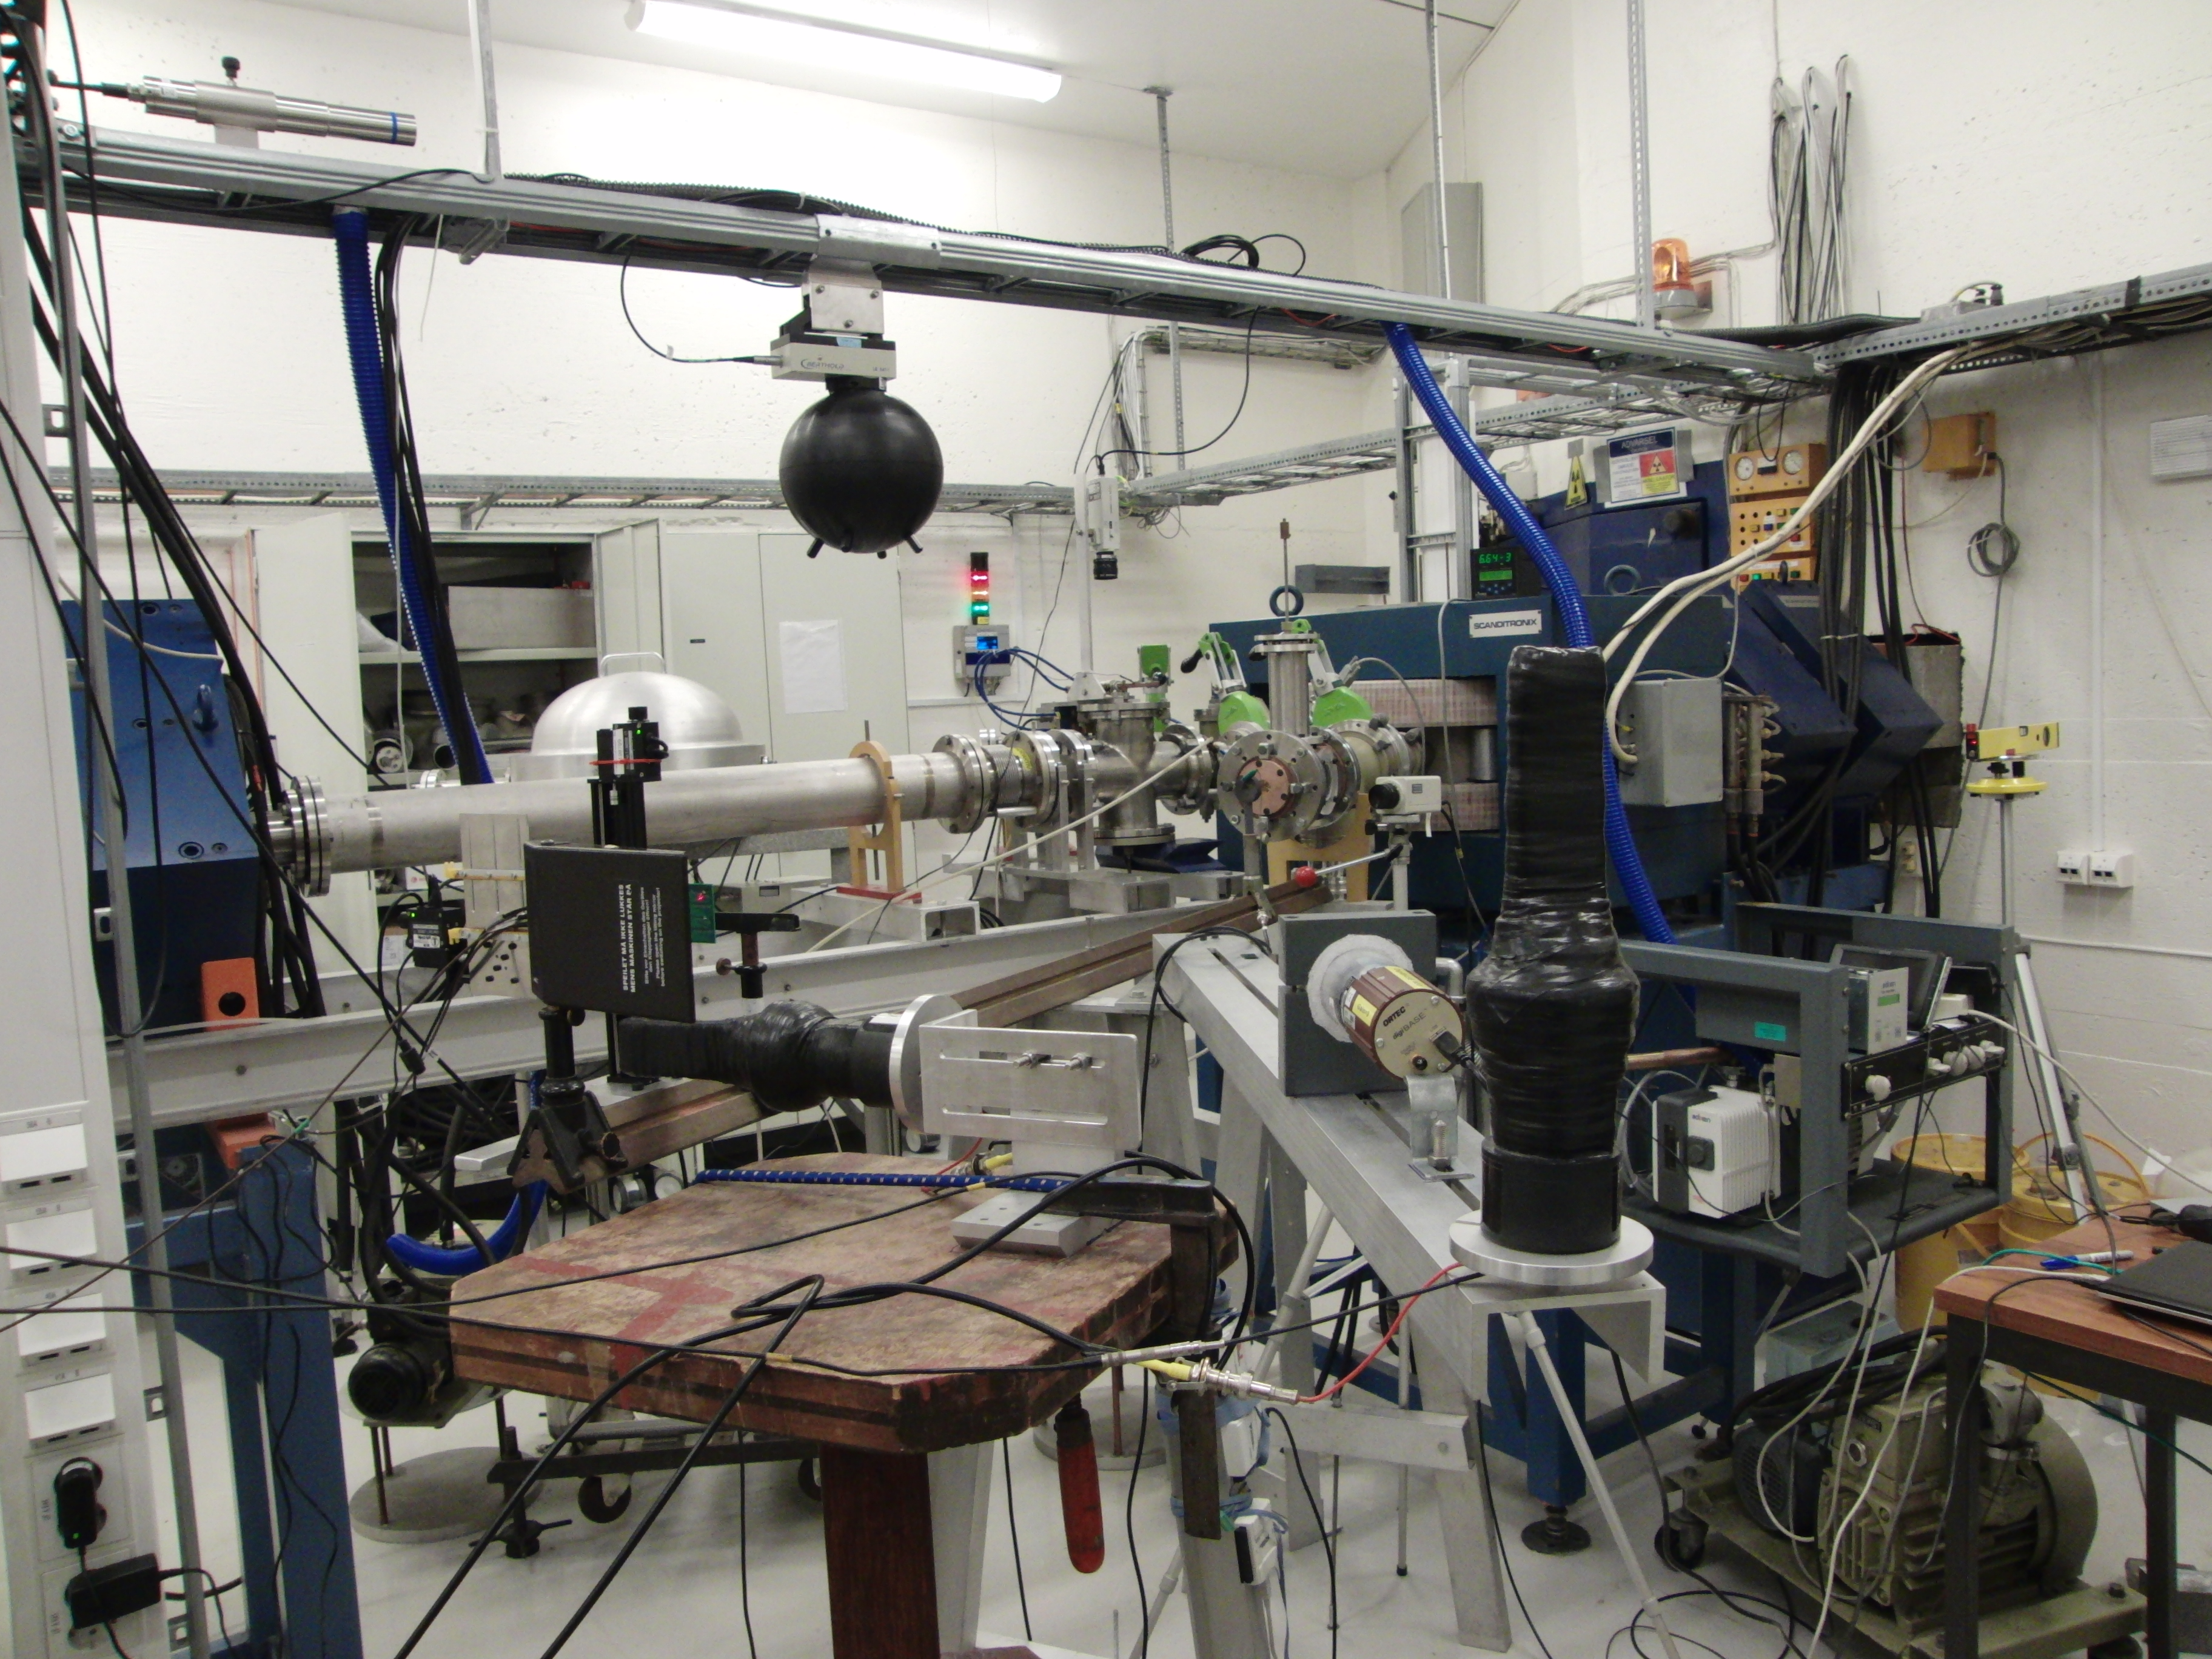
\includegraphics[width=\textwidth]{experiment_area.jpg}
  \caption{Picture of the experimental area}
  \label{experiment_area}
\end{figure}


\newpage
\begin{table}[!htbp]
 \centering
\begin{tabular}{|l|p{10cm}|}\hline
Equipment & Explanation  \\ \hline \hline
Scintillator & A plastic scintillator with photomultiplier. Was used to measure relative radiation. We had two of these, one that was placed right under DUT and one that was placed 75cm away from DUT. We only used the one 75cm away during the experiment.   \\ \hline
High voltage regulator & Voltage for the photomultiplier. 800V was used  \\ \hline
8 test boards &  TPS51200, MIC69302WU, SN74AVCB16245, SN74AVC2T245, QS3VH257, SY89831U, ADN2814 and MAX3748 \\ \hline 
SRAM-board  & A PCB board with 4 SRAM cells that was used to characterise the beam and to measure scintillator counts \\ \hline
Computer  & A VPN connection was set on a computer inside the experimental hall, so that we were able to control the experiment from the control room. The computer was running LabView to control the experiment. Data was also saved on the computer\\ \hline
USB DAQ  & Used to establish analog and digital connection to the test boards and send data to the computer. \\ \hline
Radiation film  & A film that reacts when radiated with protons. Used to identify the beam. \\ \hline
Counting controller  & A device that counts rising or falling edges of a signal. \\ \hline
leveled laser  & This was used to pinpoint the center of the beam.\\ \hline
Mirror & Used to reflect the laser beam to the backside of the test boards.\\ \hline
XY-controller  & Connected to the computer so we can do changes to the placement of the test boards from outside the experimental area\\ \hline
\end{tabular}
\caption{Equipment used in the experiment}
\label{equipment}
\end{table}

\subsection{Measurement equipment and test boards}
\subsubsection{SRAM}
The SRAM board consist of several SRAM chips and a flash based FPGA and some connections and supporting electronics. 
%A known pattern is written to the SRAM chips, and this pattern are constantly checked with the FPGA. 
When a SRAM chip is exposed to radiation a Single Event Upset(SEU) can occur.
The method of detecting an Single Event Upset (SEU) in a SRAM is rather straight
forward, as can be seen in the flow diagram of figure \ref{flowchart}. There is an initial startup
phase where a known pattern is written to all the addresses in the SRAM. When
the startup phase is done, the value from the first address is read back and compared
to a known value by xoring the known value with the read. If they are not alike a SEU has occurred,
and a 1 will return from the xor and be added to a SEU counter.
The correct value is then written back to the address and the system moves on to the next address.
  
A checkerboard pattern, a pattern of alternating ones and zeros, is used when writing
to the SRAM. To check for stuck bits, the bit pattern in the whole address space is inverted after each read. 
The cross section for SEU and particles is known through earlier experiment with the SRAM-board,
and is found to be $\unit{1.14\e{-6}}{\centi\square\meter}$.
The FPGA on the SRAM PCB is designed with RS485 two-way communication which makes it possible to edit firmware as well as sending data out. 
Through the experiment the SRAM PCB was connected with RS485 to a Opal Kelly XEM3001 that could be connected to a computer. On the computer we run a LabVIEW program, that made us able to monitor data, as well as doing some settings. 
The SRAM board also had an input for scintillator counts, so we could monitor scintillator counts by the use of this board.

\begin{figure}[!htbp]
  \centering
  \includegraphics[height=8cm, width=4cm]{SRAM_flowchart.png}
  \caption{Flowchart for SEU detection}
  \label{flowchart}
\end{figure}

In figure \ref{labview_SRAM} bellow you can see how the labVIEW program looked like. From here vi can monitor SEU on all the 4 SRAM cells, and see scintillator counts, reset counters, see time from start as well as other things. SRAM1-10 as you can see on the left side, is different SRAM-board.

\begin{figure}[!htbp]
  \centering
  \includegraphics[width=\textwidth]{SRAM_labview.png}
  \caption{LabVIEW program for the SRAM}
  \label{labview_SRAM}
\end{figure}

\FloatBarrier

\subsubsection{Scintillator counter}
A scintillator is a material that gives out light when it is exposed to ionised radiation. The detection of ionizing radiation by the scintillation light produced in certain materials is one of the oldest techniques on record. In Geiger and Marsden�s famous scattering experiment of $\alpha$-particles off Gold nuclei, the scattered $\alpha$�s were observed via the scintillation light they produced when they hit a ZnS-screen. ZnS produced light flashes, called scintillation light, when hit by an $\alpha$. The scintillation process remains one of the most useful methods available for the detection and spectroscopy of a wide assortment of radiation.
In the beginning the scintillator was used as a single instrument. By detection of light, you would know that radiation has occurred. But because of the limitations of the eye, the scintillator was outcompeted by the gas detector until the photomultiplicator-tube(PMT) was discovered in 1944.
There are several different material used as scintillator, the most common ones are NaI(T1)-detector and plastic scintillator(NE$_{102A}$).

The PM-tube works in the way that with just a slightly light from the scintillator will be converted to a photoelectron and amplified, and outputted as a current pulse at the output. By counting the numbers of pulses, we can determine number of ionized particles that hits the scintillator.\cite{rad_phys}

\begin{figure}[!htbp]
  \centering
  \includegraphics[width=\textwidth]{scintillator.png}
  \caption{Concept drawing of scintillator}
  \label{scintillator}
\end{figure}

\newpage

\subsubsection{The test boards}
Every IC that has been tested through this thesis are planed to be used at RCU2, if they pass the test. Two of the IC have the same purpose, ADN2814 and MAX3748, the one that performs best of these two will be used in the design of RCU2.

\paragraph{TPS51200} -
A power regulator, special designed for DDR RAMs. Can be used for DDR, DDR2, DDR3 and DDR4 aplications. On the RCU2 board, this IC is going to be used for 0.75V DDR3 RAM.

\paragraph{MIC69302WU} -
This is a power regulator that are able to deliver high current through low voltage. This is going to be used to produce a 1.2V voltage, and power everything that requires 1.2V on the board.

\paragraph{SN74AVCB16245} -
This is a 16-bit noninverting bus transceiver, with configurable voltage transceiver and 3-state outputs. On the RCU2 this is going to be used as a bus transceiver with 1.5V inn and 3.3V out. 

\paragraph{SN74AVC2T245} -
This is a dual-bit noninverting bus transceiver, with configurable voltage transceiver and 3-state outputs. Used to convert a 2.5V SPI signal to a 3.3V SPI signal.

\paragraph{QS3VH257} -
This is a Quad 2 to 1 multiplexer/demultiplexer with high bandwidth bus switch. Used to switch the JTAG connection between SF2 and A2P(ProASIC3 Flash).

\paragraph{SY89831U} -
This is a high speed, 2$\giga\hertz$ differential LVPECL 1 to 4 fanout buffer optimized for ultra-low skew applications. Used on the RCU2 to produce 4 clock signal for 1.

\paragraph{ADN2814} -
This i a clock and data recovery IC with integrated limiting amplifier. Works in rate of 10Mb/s to 675 Mb/s. This is going to be used to give out LVDS signal out of a optic Manchester signal.

\paragraph{MAX3748} -
This is a limiting amplifier. Works in rate of 155Mb/s to 4.25Gb/s. This is going to be used to give out LVDS signal of a optic Manchester signal. 

\subsubsection{Software}
There has been made a simple LabVIEW program for each of the IC. In this program time from start can be seen, current consumption, and the status of the output signal(or the output voltage for the regulators). You are also able to do some changes, like time between each change on the input and turn thing on and off.
In figure \ref{labVIEW} you can see an example from the labVIEW program used for SN74AVC2T245.

For ADN2814 and MAX3748 the SF2 board also had to be used to code a clock and data signal into a Manchester-signal and to decode the Manchester signal back to clock and data after it has gone through the IC. The SF2 was also used to compare the original signal with the signal coming out from the IC.
A picture of the Smart Design can be seen in figure \ref{SF2}. This consist of IP-cells from ACTEL and some VHDL code that has been made.

\begin{figure}[!htbp]
  \centering
  \includegraphics[width=\textwidth]{labVIEW.jpg}
  \caption{LabVIEW program for SN74AVC2T245}
  \label{labVIEW}
\end{figure}

\begin{figure}[!htbp]
  \centering
  \includegraphics[width=\textwidth]{vhdl_adn.png}
  \caption{Smart Design for ADN2814}
  \label{SF2}
\end{figure}

\subsubsection{X-Y-controller}
In figure \ref{xy-table} you can see how the labVIEW program controlling the XY-table. From here it is possible to control the position of the XY-table. When center of the beam was found that position could be set as x=0,y=0, and use that as a starting point when we wanted to start testing or calibration.

\begin{figure}[!htbp]
  \centering
  \includegraphics[width=\textwidth]{xy-table.jpg}
  \caption{LabVIEW program to control the X-Y-controller}
  \label{xy-table}
\end{figure}

\newpage

\subsection{Preparation and characterization of the beam}
Before testing of the boards could start, the cyclotron had to be made ready for a proton beam and the magnet controlling the direction had to be put in the right position to get the beam out in experiment area 2. This was done by the experienced lab personnel. 

\subsubsection{Purpose of tests}
The purpose of testing these board is to see if they are able to survive in a highly radiated area.
Every IC that has been tested, are IC's that are going to be used in creation of the new RCU2 board, that is going to be placed in ALICE at CERN.


\subsubsection{Beam setup}
  \label{beam_setup}
When the beam was set, we could start the characterization of the beam.
The first thing to do is to get an understanding of the beam,
too see that it is centered and that it hits around the area that we expect.
This was done by using radiation films that turns black when exposed to radiation. 
One of these was put right in front of the beam exit and one in front of DUT-area to see how the beam looks like at the two places.
This gave us a hunch of where the beam goes. A more precise calibration was done by the use of the SRAM board and the scintillator. 
By measuring the relation between scintillator counts on the scintillator which was in a locked position and SEU on the SRAM that was connected to a XY-controller(which made the SRAM freely to move), we were able to find a more precise position of the beam center by seeing which position gives most SEU compared to scintillator counts.

This had to be done everyday at startup before we could start the tests.
When the beam center is found and everything looks fine, the laser was placed in a position so the laser points to where we had found center of the beam to be. After that we could switch out the SRAM board with the PCB that we were going to test. We were able to control the intensity of the beam freely from the control room inside the limitation of the beam (for protons that is up to 100$\micro\ampere$). This way the radiation dose to the test boards can be controlled. The beam intensity could be measured with a Faraday Cup(FC), by putting one in front of the beam. But the FC had to be removed when tests were running, since it will block the beam.

\subsubsection{The test procedure}
Before the test day I had made simple test programs in LabVIEW for each PCB that we were going to test.
Each PCB had a mark on the back indicating the center of the IC, when the laser pinpoint this mark, then the IC should be in the center of the beam.
We were running 3 labVIEW programs at all time through the experiment, one for controlling the XY-controller,
one for SRAM PCB(for scintillator counts) and one program for each of the test boards.
The SRAM and test board programs were constantly saving data on the disk.

\newpage

\section{Results and calculations from beam test at OCL}
The radiation was done in 5 days divided in two periods 13.11-15.11 and 28.11-29.11. I had made two version of most of the boards, the exception is ADN2814 and MAX3748 which I only made one version of.
The boards that where tested the first time are $TPS51200_1, MIC69302WU_1, SN74AVCB16245_1, SN74AVC2T245_1,$
$QS3VH257_1$ and $SY89831U_1$ tested in that order. The first time at OCL we were given an beam of 28MeV, but the second time the lab personnel manage only to produce a beam of 25MeV.
When the beam gets out through the beam exit the energy will be reduced by crashing with air particles(~21keV per cm), so at DUT area the beam was approx ~25MeV and ~22MeV.

The result is presented after type, so that the two boards of the same type is presented together. 

\subsection{Calibration process}
As explained in chapter $\ref{beam_setup}$, we had to start with finding the center of the beam. In table $\ref{test_15.11}$ you can see the results from our calibration 15.11.2013. You can see that position x = -2,5 and y = -1 gives highest relation between SEU on the SRAM and SC. A total of 4 tests in that position was done and the average value gives us 0,0948.
This value was used to calculate from SC to SEU, since there is a known cross section(CS)(the probability that an incoming particle will induce an SEU). The CS is given in equation \ref{CS}.

% Table generated by Excel2LaTeX from sheet 'Sheet1'
\begin{table}[!htbp]
  \centering
    \begin{tabular}{|r|r|r|r|r|r|}\hline
    Calibration test nr.: & x     & y     & Scint rel & SEU(SRAM) & SEU(SRAM)/SC \\ \hline \hline
    1     & -0,8  & -1    & 27798 & 1463  & 5,26E-02 \\ \hline
    2     & -1,3  & -1    & 17721 & 1239  & 6,99E-02 \\ \hline
    3     & -1,8  & -1    & 12904 & 1203  & 9,32E-02 \\ \hline
    4     & -2,3  & -1    & 13361 & 1276  & 9,55E-02 \\ \hline
    5     & -2,8  & -1    & 12786 & 1238  & 9,68E-02 \\ \hline
    6     & -3,3  & -1    & 12342 & 1156  & 9,37E-02 \\ \hline
    7     & -2,5  & -1    & 11696 & 1223  & 1,05E-01 \\ \hline
    8     & -2,5  & -1,5  & 11027 & 1075  & 9,75E-02 \\ \hline
    9     & -2,5  & -2    & 11835 & 1063  & 8,98E-02 \\ \hline
    10    & -2,5  & -0,5  & 15593 & 1540  & 9,88E-02 \\ \hline
    11    & -2,5  & 0     & 12620 & 1034  & 8,19E-02 \\ \hline
    12    & -2,5  & -1    & 65280 & 5999  & 9,19E-02 \\ \hline
    13    & -2,5  & -1    & 52752 & 4803  & 9,10E-02 \\ \hline
    14    & -2,5  & -1    & 57229 & 5250  & 9,17E-02 \\ \hline
    \end{tabular}%
      \caption{Calibration tests 15.11.2013}
  \label{test_15.11}%
\end{table}%

\begin{equation}
scint\_conv = \frac{SEU(SRAM)} {SC} = 0,0948
\label{scint_conv}
\end{equation}

\begin{equation}
CS = 1,14e-6
\label{CS}
\end{equation}

\subsection{Test results}
The tests was controlled and monitored through a LabVIEW program for each of the different IC. When testing ADN2814 and MAX3748 there was also needed a SF2 board, to configure and monitor the input signal. A complete result of the tests can be found in one of the appendix.
The point of this test was to see that these IC's would survive in a radiated area. The total dose of 10 years in ALICE-experiment is estimated to be 0.6kRad. If a IC survives more than 10 times that, we can be quite sure that it will survive the radiation it will receive at CERN.
In table \ref{dose_15.11} and \ref{dose_28.11} you can see how long each IC has been exposed, the dose they has been received and if an error occurred.

\begin{table}[!htbp]
 \centering
\begin{tabular}{|l|l|l|l|}\hline
Device & Exposed time[s] & Dose[Rad] & Error \\ \hline \hline
$TPS51200$ & 2065 & 41800 & No \\ \hline
$MIC69302WU_1$ & 2240 & 164000 & No \\ \hline
$SN74AVCB16245_1$ & 967  & 65200 & No \\ \hline
$SN74AVC2T245_1$ & 860  & 4600 & Yes \\ \hline
$QS3VH257_1$ & 795  & 52800 & No \\ \hline
$SY89831_1$ & 1251 & 93500 & No \\ \hline
\end{tabular}
\caption{Tests at OCL 15.nov 2013}
\label{dose_15.11}
\end{table}

\begin{table}[!htbp]
 \centering
\begin{tabular}{|l|l|l|l|}\hline
Device & Exposed time[s] & Dose[Rad] &  \\ \hline \hline
$ADN2814/_run1$ & 1273 & 20200 & Yes \\ \hline
$ADN2814/_run2$ & 2286 & 324900 & Yes \\ \hline
$MAX3748$ & 2384 & 442200 & No \\ \hline
$TPS51200_2$ & -\textsuperscript{*} & -* & -* \\ \hline
$MIC69302WU_2$ & 1385 & 383800 & No \\ \hline
$SN74AVCB16245_2$ & 526  & 201400 & No \\ \hline
$SN74AVC2T245_2$ & 478  & 161600 & No \\ \hline
$QS3VH257_2$ & 264  & 110300 & No \\ \hline
$SY89831U_2$ & 921  & 165800 & No \\ \hline
\multicolumn{4}{l}{\textsuperscript{*}\footnotesize{The board wouldn't work at test time}}
\end{tabular}
\caption{Tests at OCL 27-28.nov 2013}
\label{dose_28.11}
\end{table}

\begin{figure}[!htbp]
  \centering
  \includegraphics[width=\textwidth]{flux_all_test1.jpg}
  \caption{flux for each component radiated 15.11.2013}
  \label{flux_all1}
\end{figure}

\begin{figure}[!htbp]
  \centering
  \includegraphics[width=\textwidth]{Flux_vs_time_all.jpg}
  \caption{flux for each component radiated 15.11.2013}
  \label{flux_all2}
\end{figure}
\newpage
In figure $\ref{flux_all1}$ and $\ref{flux_all2}$ you can see graphs of flux vs time for the different test boards. The reason for that graph don't go as linear, is that the beam sometimes fell out and that we increased the intensities when we saw that thing went a little slow.
\FloatBarrier

\subsubsection{TPS51200}
This was the first board that was tested. To measure the current going into the board, we added a 220$\ohm$ resistor on the input, and measured over this resistor to calculate the current.
A 3v3 voltage was supplied from the DAQs analog outputs. The output voltage was also monitored, through a analog input on the DAQ-box.
The intensity was a little low on this test. To make the testing process faster the intensity was increased during the next test.

The IC worked after a dose of 40kRad, but we could see a little increase in current after a dose of 25kRad. The output voltage is close to stable, a few mV up and down, but not noteworthy.
Two PCBs of this type was tested, but only one worked when we was at OCL to do the testing.

\begin{figure}[!htbp]
  \includegraphics[width=.45\textwidth]{current_voltage_tps.jpg}
  \caption{TPS51200 - Current/Voltage vs Dose}
  \label{TPS51200_1}
\end{figure}

\FloatBarrier

\subsubsection{MIC69302WU}
The first board was tested 15.11.13 and the second board was tested 28.11.13. During the test of the first board we increased the intensity of the beam quite allot, that can be seen from the flux graph, figure \ref{flux_all1}.
The current was measured, by adding a 220$\ohm$ resistor on the input, and measure the voltage over the resistor to calculate the current. 

This IC had an unexpected reaction to radiation. You can see from both of the graphs that the current is decreasing and voltage is increasing, normally we would expect the opposite, or at least that the current would increase.
As seen from the graph in figure \ref{MIC69302WU_both} it starts quite early to decrease in current, but as you can see it also stabilize after a while. The output voltage is mostly stable, there were a increase of ~2\% on both the tests.

\begin{figure}[!htbp]
\centering
  \begin{subfigure}{.45\textwidth}
  \centering
  \includegraphics[width=\linewidth]{current_voltage_mic.jpg}
  \caption{MIC69302WU board1}
  \label{MIC69302WU_1}
  \end{subfigure}
  \begin{subfigure}{.45\textwidth}
  \centering
  \includegraphics[width=\linewidth]{current_volt_dose_MIC.jpg}
  \caption{MIC69302WU board2}
  \label{MIC69302WU_2}
  \end{subfigure}
 \caption{MIC69302WU - Current/Voltage vs Dose}
 \label{MIC69302WU_both}
\end{figure}

\FloatBarrier

\subsubsection{SN74AVCB16245}
The current was measured in the same way as the two previously circuits, a 220$\ohm$ resistor was placed in series with power supply, and voltage over the resistor was measured and used to calculate current. To make sure that the circuit didn't drag current through the input on the chip, we used a pMOS transistor, that was connected to supply pin on Drain, to ground on Source and Gate to a digital output from the DAQ. That way the current has to come from the power supply input, and not from the digital output of the DAQ. The outputs was measured by digital inputs.

It can be seen that the characteristics on the two test board are different, the reason for this is maybe because of different output load. The reason for the ``jumps`` in current is because the output is constantly changing from on to off, with a gap of 4 seconds.
This chips is not effected by radiation before a dose of approx 40kRad. That is more than enough for the purposes we are going to use this for.

\begin{figure}[!htbp]
\centering
  \begin{subfigure}{.45\textwidth}
  \centering
  \includegraphics[width=\linewidth]{current_4245.jpg}
  \caption{SN74AVCB16245 board1}
  \label{SN74AVCB16245_1}
  \end{subfigure}
  \begin{subfigure}{.45\textwidth}
  \centering
  \includegraphics[width=\linewidth]{current_dose_42452.jpg}
  \caption{SN74AVCB16245 board2}
  \label{SN74AVCB16245_2}
  \end{subfigure}
 \caption{SN74AVC2T245 - Current vs Dose}
\end{figure}

\FloatBarrier

\subsubsection{SN74AVC2T245}
This chip is almost the same as the SN74AVCB16245. A 220$\ohm$ resistor was used at the input to measure current, a digital output from the DAQ was used to put the input high and low, and digital inputs was used to measure the outputs.

Something went wrong on the first test. After 740s and a dose of 98Rad the chips output was stuck at 1. The reason for this is unknown, I fear that this might be defected before we started the test, since it gives a totally different characteristics than test board nr2.
The input was switching from high to low every 4 second. If we look at the test results from board 2. the current goes unchanged up to 40kRad, and that is more than enough.
%her m� eg sjekke board1 etter eg har f�tt den tilbake, og se om den faktisk fungere. Kan hende at denne har v�rt �delagt f�r vi begynte.

\begin{figure}[!htbp]
\centering
  \begin{subfigure}{.45\textwidth}
  \centering
  \includegraphics[width=\linewidth]{current_t245.jpg}
  \caption{SN74AVC2T245 board1}
  \label{SN74AVC2T245_1}
  \end{subfigure}
  \begin{subfigure}{.45\textwidth}
  \centering
  \includegraphics[width=\linewidth]{current_dose_t2452.jpg}
  \caption{SN74AVC2T245 board2}
  \label{SN74AVC2T245_2}
  \end{subfigure}
 \caption{SN74AVC2T245 - Current vs Dose}
\end{figure}

\FloatBarrier

\subsubsection{QS3VH257}
This was also tested by putting a 220$\ohm$ resistor in series with the power supply, in the same way as the others. For the Select input a analog output signal from the DAQ was used. The input signals was set by digital outputs from the DAQ. The outputs was measured by digital inputs on the DAQ.
The select input was changed every 4 second and the inputs was changed every 18second.

Both of the boards worked fine through the tests. 
We see that we have small increase in current before 30kRad, after that it increases quite allot. We couldn't see any errors on the output during the experiment, but it should probably not be exposed to more than 30kRad.

\begin{figure}[!htbp]
\centering
  \begin{subfigure}{.45\textwidth}
  \centering
  \includegraphics[width=\linewidth]{current_q.jpg}
  \caption{QS3VH257 board1}
  \label{QS3VH257_1}
  \end{subfigure}
  \begin{subfigure}{.45\textwidth}
  \centering
  \includegraphics[width=\linewidth]{current_dose_q2.jpg}
  \caption{QS3VH257 board2}
  \label{QS3VH257_2}
  \end{subfigure}
 \caption{QS3VH257 - Current vs Dose}
\end{figure}

\FloatBarrier

\subsubsection{SY89831}
This is a buffer used to make 1 clock to 4 clocks. This chip required a high current to work, and since the labVIEW DAQ box only delivers 5mA on the analog outputs, I had to use the 5V output on the DAQ that could deliver up to 200mA. But I also needed to have a 3v3 power supply, this was solved by using a modified MIC69302WU board to supply this IC. To measure the current, I had to use 20$\ohm$ resistor to make sure that I didn't had a voltage drop, because of the high current consumption. voltage over this resistor was measured to get current.
To test that the chip worked as it should, two analog outputs from the DAQ was used to make a DC differential input. This was measured by digital inputs on a DAQ to see that i goes high and low according to the input.

A difference in characteristics can also be seen here. This maybe because two different footprint for the PCB was used, and therefor the component are different placed on the PCB. We see a small increase in current on both of the boards, but not noteworthy, compared to how much current this IC is using.


\begin{figure}[!htbp]
\centering
  \begin{subfigure}{.45\textwidth}
  \centering
  \includegraphics[width=\linewidth]{current_sy.jpg}
  \caption{SY89831 board1}
  \label{SY89831_1}
  \end{subfigure}
  \begin{subfigure}{.45\textwidth}
  \centering
  \includegraphics[width=\linewidth]{current_dose_SY2.jpg}
  \caption{SY89831 board2}
  \label{SY89831_2}
  \end{subfigure}
 \caption{SY89831 - Current vs Dose}
\end{figure}

\FloatBarrier

\subsubsection{ADN2814}
This IC is a little special and was hard to get a good test on. This is a clock and data return circuit, with a limiting amplifier.
The SF2 board was used to code a clock and data into a differential Manchester signal, that was sent into the IC. Out of the IC we get a clock and a limited Manchester coded data signal. The Mancheseter coded data signal was decoded on the Igloo FPGA on SF2 board, so that we get out a clock and data. The data was tested by delaying the original data through a few D-latches, so that the original and returned data was close to alike. Then we could compare the original data with the one from the chip through a XOR-function, to see if they was alike. This function was triggered by a 80Mhz clock from the SF2 board. If they aren't alike when the clock rises, a 1 was added to a counter. The value of the counter was constantly sent through the UART of the SF2 board.

The way the clock was tested was a little harder process since the clock was so fast(160Mhz).
This was solved, was by adding a third clock with the same frequency(160Mhz) that was $90\,^{\circ}$ of from the two others, when this goes high I called on the XOR-function, to see if the two other clocks are the same. if they are alike, nothing happens, if they are not the program adds 1 to a counter, which constantly writes its current value to a UART.
The problem here is that for each time the SF2 board was programed the clock was slightly different, that made either the clock out of sync or the data out of sync, so that the code didn't work as it should.
This circuit also requires allot of current, therefore the same solution as for SY89831 was used, using MIC69302WU as a power supply and measure the current on that PCB.

The current didn't change before a dose of 200kRad had been received, but we got a clock error at a dose of ~11kRad, and a data error after a dose of ~8kRad.
How good this test really is, could be discussed, since we don't have any data on the clock and data, other than that the XOR-function failed. What really failed, and how much is impossible to know. It could be a slightly delay on a clock or the data, or maybe the clock just disappeared for a moment. There could also be a problem with the clocks on the SF2 board.

\begin{figure}[!htbp]
\centering
  \begin{subfigure}{.45\textwidth}
  \centering
  \includegraphics[width=\linewidth]{current_dose_ADN_t1.jpg}
  \caption{ADN2814 test1}
  \label{ADN2814_1}
  \end{subfigure}
  \begin{subfigure}{.45\textwidth}
  \centering
  \includegraphics[width=\linewidth]{current_dose_ADN_t2.jpg}
  \caption{ADN2814 test2}
  \label{ADN2814_2}
  \end{subfigure}
 \caption{ADN2814 - Current vs Dose}
\end{figure}

\begin{figure}[!htbp]
\centering
  \begin{subfigure}{.45\textwidth}
  \centering
  \includegraphics[width=\linewidth]{error_dose_ADN_t1.jpg}
  \caption{ADN2814 test1}
  \label{ADN2814_1e}
  \end{subfigure}
  \begin{subfigure}{.45\textwidth}
  \centering
  \includegraphics[width=\linewidth]{error_dose_ADN_t2.jpg}
  \caption{ADN2814 test2}
  \label{ADN2814_2e}
  \end{subfigure}
 \caption{ADN2814 - Relative errors vs Dose}
\end{figure}

\FloatBarrier

\subsubsection{MAX3748}
This circuit has the same purpose as ADN2814, the difference is that this one only return the limited Manchester coded signal, and no clock. The process for testing the data is the same as for the ADN2814.
The decoding process return clock and data, but since they are related to another, a error on the clock would mean an error at the data. So by measuring data, we can be sure that there are no clock errors as well. 

After a dose of over 400kRad this chip still worked, and current consumption was stable through the hole radiation process.

\begin{figure}[!htbp]
\centering
  \begin{subfigure}{.45\textwidth}
  \centering
  \includegraphics[width=\linewidth]{current_dose_MAX.jpg}
  \caption{Current vs Dose}
  \label{MAX3748}
  \end{subfigure}
  \begin{subfigure}{.45\textwidth}
  \centering
  \includegraphics[width=\linewidth]{error_dose_MAX.jpg}
  \caption{Errors vs Dose}
  \label{MAX3748_error}
  \end{subfigure}
 \caption{MAX3748}
\end{figure}

\FloatBarrier

\newpage

\subsection{Calculation of dose}
After a radiation test on one of the PCB, we knew the exposed time and scintillator counts(SC). From the calibration we knew the relation between scintillator counts and SEU on the SRAM, and cross section(CS). 
We start by calculating SEU from the factor given in equation $\ref{scint_conv}$. Then we calculate the fluence at DUT as seen in equation $\ref{FluenceDUT}$, and by this we can calculate the flux, see equation $\ref{flux}$.
To calculate the dose from here we need to know some more factors. We run a simulation on a program called FLUKA. This program is used to simulate particles in different environment. We simulated a proton beam of 28MeV and 25MeV, and inserted the distance from BE(Bean exit). The results can be seen in table $\ref{FLUKA_15}$.
Then we had enough information to calculate the dose. As seen from equation $\ref{FluenceBE}$ we are able to find the Fluence at BE. And from there we can calculate the dose at DUT, see equation \ref{DoseDUT}.


% Table generated by Excel2LaTeX from sheet 'Fluka'
\begin{table}[!htbp]
  \centering
    \begin{tabular}{|l|l|} \hline
    Fluka simulation results 28MeV &  \\\hline\hline
    Dose/primary particle at DUT[Gy] & 4,08E-10 \\\hline
    Primary particles at Beam exit & 1 \\\hline
    Primary particles at DUT & 0,1331 \\\hline
    Beam intensity reduction  at DUT & 7,513148009 \\\hline
    \end{tabular}%
      \caption{FLUKA simulation with 28MeV proton beam}
  \label{FLUKA_15}%
\end{table}%


\begin{equation}
FluenceDUT = \frac{SEU}{CS}
\label{FluenceDUT}
\end{equation}

\begin{equation}
Flux = \frac{Fluence}{time}
\label{flux}
\end{equation}

\begin{equation}
FluenceBE = \frac{fluenceDUT}{primary_particlesDUT}
\label{FluenceBE}
\end{equation}

\begin{equation}
DoseDUT[Gy] = FluenceBE * \frac{Dose}{primary particle at DUT}
\label{DoseDUT}
\end{equation}

\begin{equation}
1 Rad = 100 Gy
\label{Gy_to_Rad}
\end{equation}

\newpage
\subsection{Discussion of the result}
Most of the testing was done the 15.nov and 28.nov. The other days was used to get too know the instruments and equipment being used, to prepare the setup and setting up the beam.
There are almost impossible to get the same beam two days at a row. Each day of testing is therefore different from each other. Since the testing was conducted in two periodes and a total of 4 test days, there are allot of uncertainties regarding the beam.
And that is also why we had to do calibration each day at start-up.

When we where going to measure the intensity at the BE, we placed a faraday cup in front of the beam, and connected it to a amperemeter on the kontroll panel, but since the current is so small, the measuring instrument will be affected by air currents, and there are also allot of uncertainties in the instruments. Therefore we only used the FC, to get a hunch of the actual intensity.

The are also some uncertainties regarding the DAQ box form NI. When measuring digital signal, we don't know if it goes from 0V to 3v3V as we would expect. Maybe in reality the low voltage is actually 0.4V and high voltage is actually 2.8V. If this is the case, it could be a problem with using this in our design.

As said before in \ref{beam_setup}, if a component survives 10 times more than what it will receive in a period of 10 years in ALICE, that is 0.6kRad, than it can be used in the design of RCU2.
Having that in mind, I would say that every component tested would have a green flag even though we had some errors when testing SN74AVC2T245 and ADN2814. Since the result after testing board two of SN74AVC2T245, was positive we can assume that something was wrong with the first board. When it comes to ADN2814, I would rather have time to test this even more, since the test done gave us so unclear results. But it manage to run error free until a dose of 8kRad, and that is more than enough for our use.
Some of the tests gave us some unclear results, and if we had more time and chances to use to lab it would have been nice to do some more testing.

\newpage

\section{Conclusion}


\newpage
\FloatBarrier

\section{Appendix}

% Table generated by Excel2LaTeX from sheet 'Sheet1'
\begin{table}
  \centering
    \begin{tabular}{|l|l|l|l|l|l|} \hline
    Calibration test nr.: & x     & y     & Scint rel & SEU(SRAM) & SEU(SRAM)/SC \\ \hline \hline
    1     & 0     & 0     & 23813 & 1971  & 8,28E-02 \\ \hline
    2     & 0     & -0,5  & 37930 & 3867  & 1,02E-01 \\ \hline
    3     & 0     & -1    & 27527 & 2817  & 1,02E-01 \\ \hline
    4     & 0     & -1,5  & 34413 & 3360  & 9,76E-02 \\ \hline
    5     & 0     & -2    & 32713 & 2763  & 8,45E-02 \\ \hline
    6     & 0,5   & 0     & 38753 & 2709  & 6,99E-02 \\ \hline
    7     & -0,5  & 0     & 23420 & 2483  & 1,06E-01 \\ \hline
    8     & -1    & 0     & 20611 & 2232  & 1,08E-01 \\ \hline	
    9     & -1,5  & 0     & 21014 & 2410  & 1,15E-01 \\ \hline
    10    & -1,5  & 0     & 20676 & 2260  & 1,09E-01 \\ \hline
    11    & -2    & 0     & 35787 & 3776  & 1,06E-01 \\ \hline
    12    & -2,5  & 0     & 27847 & 2512  & 9,02E-02 \\ \hline
    \end{tabular}%
      \caption{Calibration tests 14.11.2013}
      \label{test_14.11}
\end{table}%

% Table generated by Excel2LaTeX from sheet 'Sheet1'
\begin{table}
  \centering
    \begin{tabular}{|l|l|l|l|l|l|}\hline
    Calibration test nr.: & x     & y     & Scint rel & SEU(SRAM) & SEU(SRAM)/SC \\ \hline \hline
    1     & -0,8  & -1    & 27798 & 1463  & 5,26E-02 \\ \hline
    2     & -1,3  & -1    & 17721 & 1239  & 6,99E-02 \\ \hline
    3     & -1,8  & -1    & 12904 & 1203  & 9,32E-02 \\ \hline
    4     & -2,3  & -1    & 13361 & 1276  & 9,55E-02 \\ \hline
    5     & -2,8  & -1    & 12786 & 1238  & 9,68E-02 \\ \hline
    6     & -3,3  & -1    & 12342 & 1156  & 9,37E-02 \\ \hline
    7     & -2,5  & -1    & 11696 & 1223  & 1,05E-01 \\ \hline
    8     & -2,5  & -1,5  & 11027 & 1075  & 9,75E-02 \\ \hline
    9     & -2,5  & -2    & 11835 & 1063  & 8,98E-02 \\ \hline
    10    & -2,5  & -0,5  & 15593 & 1540  & 9,88E-02 \\ \hline
    11    & -2,5  & 0     & 12620 & 1034  & 8,19E-02 \\ \hline
    12    & -2,5  & -1    & 65280 & 5999  & 9,19E-02 \\ \hline
    13    & -2,5  & -1    & 52752 & 4803  & 9,10E-02 \\ \hline
    14    & -2,5  & -1    & 57229 & 5250  & 9,17E-02 \\ \hline
    \end{tabular}%
      \caption{Calibration tests 15.11.2013}
\end{table}%

% Table generated by Excel2LaTeX from sheet 'Fluka'
\begin{table}
  \centering
    \begin{tabular}{|l|l|} \hline
    Fluka simulation results 28MeV &  \\\hline\hline
    Dose/primary particle at DUT[Gy] & 4,08E-10 \\\hline
    Primary particles at Beam exit & 1 \\\hline
    Primary particles at DUT & 0,1331 \\\hline
    Beam intensity reduction  at DUT & 7,513148009 \\\hline
    \end{tabular}%
      \caption{FLUKA simulation with 28MeV proton beam}
\end{table}%

% Table generated by Excel2LaTeX from sheet 'Fluka'
\begin{table}
  \centering
    \begin{tabular}{|l|l|}\hline
    Fluka simulation results 25MeV &  \\\hline\hline
    $\frac{Dose}{primary particle at DUT}$[Gy] & 2,94E-10 \\\hline
    Primary particles at Beam exit & 1 \\\hline
    Primary particles at DUT & 8,57E-02 \\\hline
    Beam intensity reduction  at DUT & 11,6713352 \\\hline
    \end{tabular}%
    \caption{FLUKA simulation with 25MeV proton beam}
  \label{FLUKA_28}%
\end{table}%


\FloatBarrier

\newpage
\bibliographystyle{plain}
\bibliography{Master_Thesis_Inge_Nikolai_Torsvik}
\end{document}